%%
%% This is file `sample-manuscript.tex',
%% generated with the docstrip utility.
%%
%% The original source files were:
%%
%% samples.dtx  (with options: `manuscript')
%%
%% IMPORTANT NOTICE:
%%
%% For the copyright see the source file.
%%
%% Any modified versions of this file must be renamed
%% with new filenames distinct from sample-manuscript.tex.
%%
%% For distribution of the original source see the terms
%% for copying and modification in the file samples.dtx.
%%
%% This generated file may be distributed as long as the
%% original source files, as listed above, are part of the
%% same distribution. (The sources need not necessarily be
%% in the same archive or directory.)
%%
%% The first command in your LaTeX source must be the \documentclass command.
%%%% Small single column format, used for CIE, CSUR, DTRAP, JACM, JDIQ, JEA, JERIC, JETC, PACMCGIT, TAAS, TACCESS, TACO, TALG, TALLIP (formerly TALIP), TCPS, TDSCI, TEAC, TECS, TELO, THRI, TIIS, TIOT, TISSEC, TIST, TKDD, TMIS, TOCE, TOCHI, TOCL, TOCS, TOCT, TODAES, TODS, TOIS, TOIT, TOMACS, TOMM (formerly TOMCCAP), TOMPECS, TOMS, TOPC, TOPLAS, TOPS, TOS, TOSEM, TOSN, TQC, TRETS, TSAS, TSC, TSLP, TWEB.
% \documentclass[acmsmall]{acmart}

%%%% Large single column format, used for IMWUT, JOCCH, PACMPL, POMACS, TAP, PACMHCI
% \documentclass[acmlarge,screen]{acmart}

%%%% Large double column format, used for TOG
\documentclass[acmtog, authorversion]{acmart}

%%%% Generic manuscript mode, required for submission
%%%% and peer review
%\documentclass[manuscript,screen,review]{acmart}

%%
%% \BibTeX command to typeset BibTeX logo in the docs
\AtBeginDocument{%
  \providecommand\BibTeX{{%
    \normalfont B\kern-0.5em{\scshape i\kern-0.25em b}\kern-0.8em\TeX}}}

%% Rights management information.  This information is sent to you
%% when you complete the rights form.  These commands have SAMPLE
%% values in them; it is your responsibility as an author to replace
%% the commands and values with those provided to you when you
%% complete the rights form.
%\setcopyright{acmcopyright}
%\copyrightyear{2018}
%\acmYear{2018}
%\acmDOI{10.1145/1122445.1122456}

%% These commands are for a PROCEEDINGS abstract or paper.
%\acmConference[Woodstock '18]{Woodstock '18: ACM Symposium on Neural
%  Gaze Detection}{June 03--05, 2018}{Woodstock, NY}
%\acmBooktitle{Woodstock '18: ACM Symposium on Neural Gaze Detection,
%  June 03--05, 2018, Woodstock, NY}
%\acmPrice{15.00}
%\acmISBN{978-1-4503-XXXX-X/18/06}


%%
%% Submission ID.
%% Use this when submitting an article to a sponsored event. You'll
%% receive a unique submission ID from the organizers
%% of the event, and this ID should be used as the parameter to this command.
%%\acmSubmissionID{123-A56-BU3}

%%
%% The majority of ACM publications use numbered citations and
%% references.  The command \citestyle{authoryear} switches to the
%% "author year" style.
%%
%% If you are preparing content for an event
%% sponsored by ACM SIGGRAPH, you must use the "author year" style of
%% citations and references.
%% Uncommenting
%% the next command will enable that style.
%%\citestyle{acmauthoryear}

%%
%% end of the preamble, start of the body of the document source.
\begin{document}

%%
%% The "title" command has an optional parameter,
%% allowing the author to define a "short title" to be used in page headers.
\title{How is testing related to Single Statement Bugs?}

%%
%% The "author" command and its associated commands are used to define
%% the authors and their affiliations.
%% Of note is the shared affiliation of the first two authors, and the
%% "authornote" and "authornotemark" commands
%% used to denote shared contribution to the research.
\author{Habibur Rahman}
\authornote{Both authors contributed equally to this research.}
\email{habibur@ualberta.ca}
\author{Saqib Ameen}
\authornotemark[1]
\email{saqib1@ualberta.ca}
\affiliation{%
  \institution{University of Alberta}
  \city{Edmonton}
  \state{AB}
  \country{CA}
}


%%
%% By default, the full list of authors will be used in the page
%% headers. Often, this list is too long, and will overlap
%% other information printed in the page headers. This command allows
%% the author to define a more concise list
%% of authors' names for this purpose.
%\renewcommand{\shortauthors}{Trovato and Tobin, et al.}

%%
%% The abstract is a short summary of the work to be presented in the
%% article.
%\begin{abstract}
%  A clear and well-documented \LaTeX\ document is presented as an
%  article formatted for publication by ACM in a conference proceedings
%  or journal publication. Based on the ``acmart'' document class, this
%  article presents and explains many of the common variations, as well
%  as many of the formatting elements an author may use in the
%  preparation of the documentation of their work.
%\end{abstract}

%%
%% The code below is generated by the tool at http://dl.acm.org/ccs.cfm.
%% Please copy and paste the code instead of the example below.
%%
%\begin{CCSXML}
%<ccs2012>
% <concept>
%  <concept_id>10010520.10010553.10010562</concept_id>
%  <concept_desc>Software Testing</concept_desc>
%  <concept_significance>500</concept_significance>
% </concept>
% <concept>
%  <concept_id>10010520.10010575.10010755</concept_id>
%  <concept_desc>Software Quality</concept_desc>
%  <concept_significance>300</concept_significance>
% </concept>
%</ccs2012>
%\end{CCSXML}

%\ccsdesc[500]{Computer systems organization~Embedded systems}
%\ccsdesc[300]{Computer systems organization~Redundancy}
%\ccsdesc{Computer systems organization~Robotics}
%\ccsdesc[100]{Networks~Network reliability}

%%
%% Keywords. The author(s) should pick words that accurately describe
%% the work being presented. Separate the keywords with commas.
%\keywords{datasets, neural networks, gaze detection, text tagging}


%%
%% This command processes the author and affiliation and title
%% information and builds the first part of the formatted document.
\maketitle

\section{Introduction}
%i. Problem Statement
Writing unit tests is a common practice in industry to ensure software quality. Usually meeting a
certain criteria of test coverage serves as a segway to product release. This is essential because software systems are used in critical areas such as health, security, finance, and space missions. In such settings, a faulty system is not acceptable. International Organization for Standardization (ISO) also mandates testing as a part of software development life cycle. Despite all efforts, the software system may still remain prone to the bugs. Which raises question on the effectiveness of testing. Is it even useful?

Multiple studies tried to answer this question under different settings but there seems to be no consensus on it. These studies examined all types of bugs that were found the in the systems. Nobody studied the effectiveness of testing on subsets of the bugs found in the software systems. One important subset of bugs is known as Single Statement Bugs (SSBs). They appear in just a single statement and can be fixed by modifying that statement. Those modifications can be as simple as changing a variable name, ordering arguments in a function, changing the return type, and so on. Figure \ref{fig:ssb} shows an example of a single statement bug where $!=$ needs to be replaced with $==$.

\begin{figure}[h]
	\begingroup
	\fontsize{7pt}{10pt}\selectfont
	\begin{verbatim}
	-   if (submittedNode == null || submittedNode.get("values") != null) {
	+   if (submittedNode == null || submittedNode.get("values") == null) {
	\end{verbatim}
	\endgroup
	\caption{Example of a single statement bug before and after the fix}
	\label{fig:ssb}
\end{figure}

SSBs occur quite often \cite{ManySStuBs4JCorpus2019} and can be very critical. For example, Apple’s return bug resulted in invalid SSL/TLS connection verification, putting the sensitive data of millions at risk. The normal distribution of the ratio of SSB/all bugs for top 100 open source java projects using Maven build system on GitHub has a bell curve show in the Figure \ref{fig:density}. We can see that the mean lies around > 0.4. Which means there are more than 40\% of SSBs in those projects. Mitigating this large chunk of bugs can be useful in improving the overall quality of the software and prevent failures in production. The goal of our study to help practitioners understand effectiveness of testing for SSBs.

\begin{figure}[h]
	\centering
	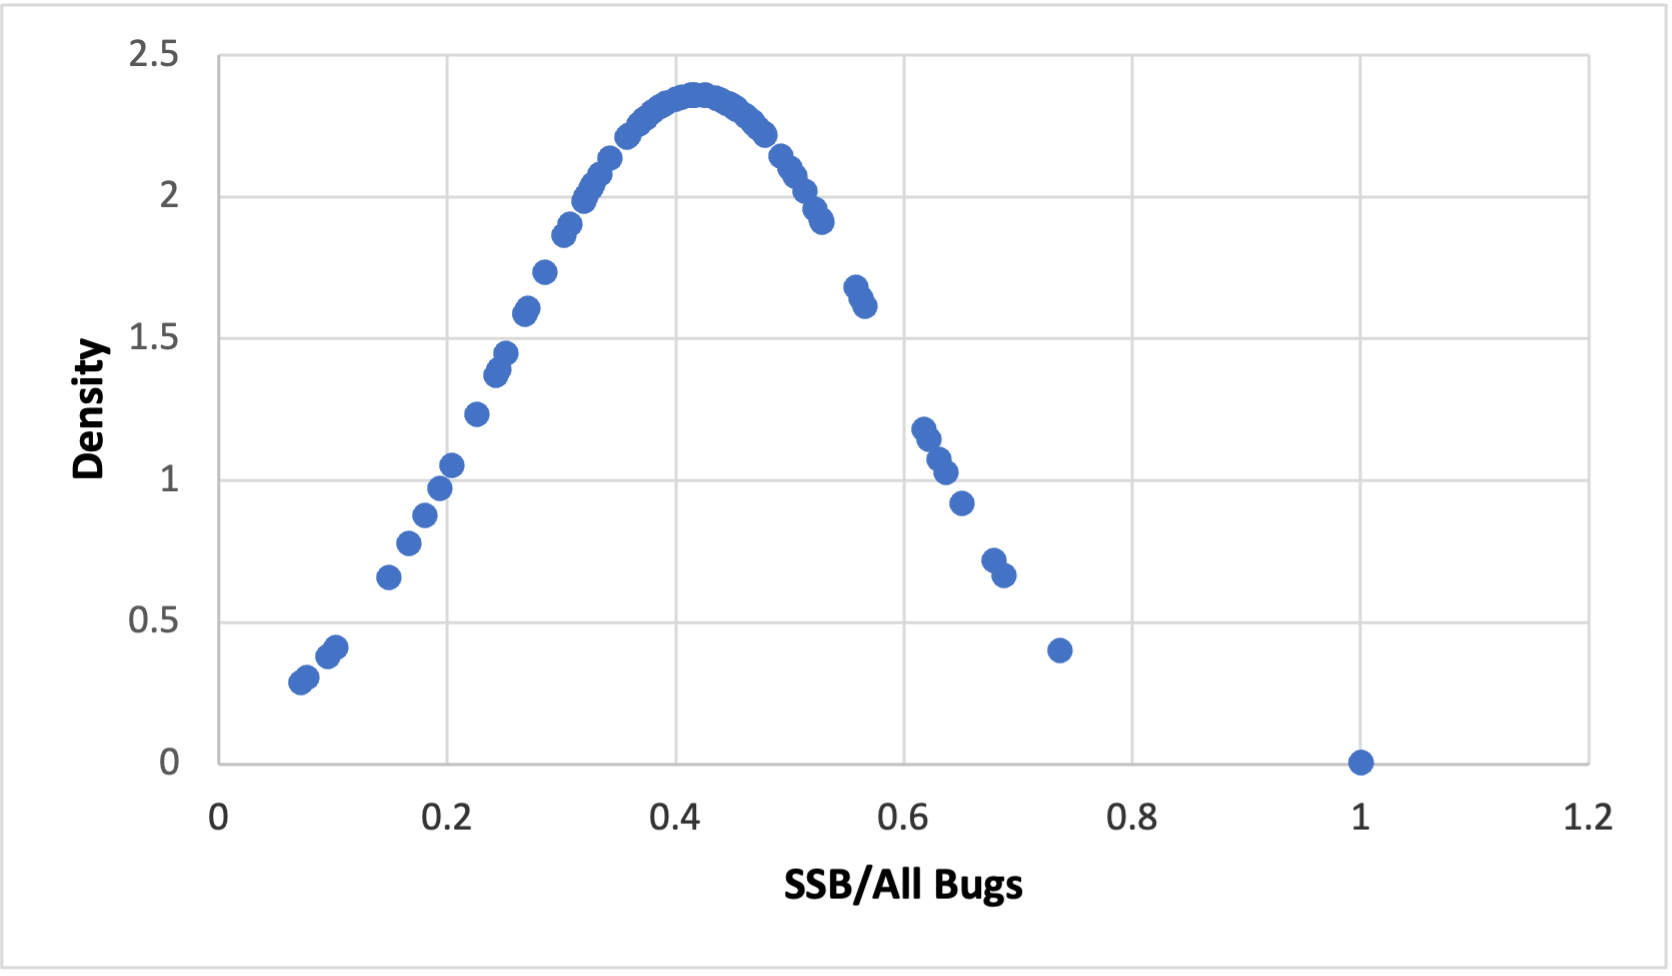
\includegraphics[width=\linewidth]{img/occurrence_of_stub.png}
	\caption{Distribution of SSBs in the top 100 open source Java projects on GitHub using Maven build system}
	\Description{A graph of density of single statement bugs}
	\label{fig:density}
\end{figure}


%iii. Research Question
We intend to understand the effectiveness of testing on SSBs by the correlation between test coverage and single statement bugs. If more test coverage in a project results in less SSBs, it shows that testing is helpful and vice versa. Which leads to our research question, \emph{Is there a correlation between test coverage and single statement bugs?} We hypothesized that there is a weak to moderate relationship between SSBs and test coverage, i.e., testing is helpful to some extent.

%iv. Summary of Methodology
To verify our hypothesis, we analyze the the post-unit test bugs in the areas covered and not covered by the testing. If a part is covered by testing, it means it has beem executed it for its intended purpose and it works fine. In future, if bugs are found in the covered part, it will show that testing did not help here. To check that, we first generate the coverage report at the release time, and see if the bugs found after the release are in covered part or not covered part. Finally, we calculate the percentage of coverage and percentage bugs in the not covered part, to find the correlation between them. It serves as a proxy for the effectiveness of unit testing for SSBs.

For our study we use the Mining Software Repositories (MSR) 2021 challenge' SSBs dataset\cite{ManySStuBs4JCorpus2019}. It contains 7824 SSBs from top 100 Maven based open source Java projects on GitHub. The important thing about this dataset is that projects can be built and their test can be executed. Which is important for us to be able to generate reports.

%v. Explicit list of Contribution
After the experiment, we have found that there is a weak to moderate correlation between the test coverage and SSBs. Which shows that testing is effective to some extent in reducing the SSBs.



\section{Background and Terminology}

%ii. Test Coverage
Test coverage is the percentage of lines of code executed by the tests for a project. We measure testing in the form of test coverage. A project that has 87\% coverage means 87 out of 100 lines of code has been executed by the test cases of that project. In this writing, the word 'coverage' refers to test coverage.

%iii. Correlation
In statistics, correlation is the statistical relationship between two random variables or bivariate data. Correlation is measured in terms of the correlation coefficient that ranges from -1 to 1 where -1 means negative correlation, 0 means no correlation, and 1 means a positive correlation between two variables. The correlation coefficient is useful for hypothesis testing. Based on the value of the correlation coefficient, a hypothesis can be accepted or rejected. There are several methods to calculate this coefficient, Pearson correlation coefficient is one of them. It can be expressed as the equation below:
\begin{equation}
r_{xy} = \dfrac{\sum{(x_{i}-\bar{x})(y_{i}-\bar{y})}}{\sqrt{\sum{{(x_{i}-\bar{x})}^{2}{(y_{i}-\bar{y})}^{2}}}}
\label{eq:1}
\end{equation}
Where:

$r_{xy}$ – the correlation coefficient of the linear relationship between the variables x and y

$x_{i}$ – the values of the x-variable in a sample

$\bar{x}$– the mean of the values of the x-variable

$y_{i}$ – the values of the y-variable in a sample

$\bar{y}$ – the mean of the values of the y-variable


Percentage test coverage and number of bugs in the not covered part are the variable for our case.


\section{Related Work}

Our work overlaps with two niches of the software engineering literature. First one is related to analyzing the relation of test coverage and its effectiveness. They utilize different techniques, under different conditions to study the usefulness of test coverage. The second one is related to the usage of SSB for an empirical study or a software application.

In the first kind of work, more or less, researchers aim to find the correlation between test coverage and the occurrence of bugs. To date, no consensus exists in the community on the usefulness of test coverage. Some studies tend to agree, while others disagree. For example, Gren and Antinyan \cite{gren_2017} and Antinyan et al.  \cite{ericson} found a weak to no correlation between the test coverage and post-unit test defects in their separate studies and concluded that test coverage was not helpful. Both of them conducted the study on a single, but large-scale industrial project. The former one did not reveal the details of the project, while the latter one worked with Ericson. Ericson mainly deals with telecommunications and networking software around the world. One aspect of these studies which is similar to our work is that they rely on actual bugs found after unit tests and real test cases written by developers. In contrast to our case, both of them considered all types of bugs, not just the SSBs. The methodology of Gren and Antinyan \cite{gren_2017} also differs from our approach, they evaluate coverage in terms of files and only consider the files with either 100\% coverage or no coverage at all. While Antinyan et al. \cite{ericson} considered the overall coverage, which is similar to our approach. Due to the small sample size and specific software niche, the results of both studies cannot be generalized for other studies.

On the other end of the spectrum, Inozemtseva and Holmes \cite{waterloo} found a weak to moderate correlation between the test coverage and its effectiveness, when the test suite size was controlled for. They conducted the study on five large open-source Java projects powered by the Ant build system and during the study. Contrary to our study, they used synthetic test suits and mutation testing to generate faulty programs. While they are a good approximation, they do not necessarily reflect the real scenarios and are limited by the algorithms behind those tools. Furthermore, they considered an extra variable, i.e., the test suite size, and varied it throughout the study while generating test cases. In our approach, we do not rely on any tests or bug generators. In another study, Namin and Andrews \cite{waterloo2} also considered the role of test suite size in addition to the coverage on the effectiveness of unit tests. They found that by increasing the coverage, indirectly, the test suite size is increased, which increases the effectiveness of tests. For varying, but controlled test suite sizes, they found a high to weak correlation between the coverage and test effectiveness. Similar to the aforementioned study, they also relied on self-generated test cases and considered only the Siemen suite of seven (C, C++) programs. Our technique is similar to what Bach et al. \cite{similar} have used in their study related to the impact of coverage on bug density. But we use a simpler approach since we only have SSBs. In comparison to our study, they considered all types of bugs and analyzed a single project, i.e., SAP HANA, and found a positive impact of coverage on bugs density. In general, the literature work on this topic differs from our work in one or more of the following areas:
\begin{itemize}
	\item A very small number of projects were considered.
	\item Artificially generated test cases were used.
	\item Synthetic bugs were introduced in the system.
	\item All types of bugs were considered.
\end{itemize}

Furthermore, in studies, done in collaboration with the industry, the details of the analyzed software were not released. Which is a barrier in generalizing or understanding the results from those studies. There could be additional internal factors and software engineering practices leading to those results. Lastly, our dataset differs from those used in the aforementioned studies.

The second part of the literature, which uses SSB mainly differs from our work in terms of intended implicatications. To the best of our knowledge, at this point, the use of SSB in literature is limited to program repair. There is no study related to test coverage and its effectiveness. Chen et al. \cite{sequenceR} used a combination of Bugs2Fix \cite{bugs2fix} and CodRep \cite{coderep} single statement dataset to propose a novel learning-based program repair technique. Their dataset is also different from the one we are using. Their dataset is not intended for building projects or running tests as there is no information on the project's build system or even if they can be run or not. Those factors are important for us to be able to generate the coverage reports. Another study by Karampatsis and Sutton \cite{sstubs} also uses SSBs. In their study, they provided a new dataset on SSBs and all types of bugs in the top 100 open-source Java projects on GitHub and attempted to find the frequency of occurrence of SSBs. They found out that SSBs occur with a frequency of one bug per 1600-2500 lines of code. Even more important contribution of this paper is that the projects in their dataset use the Maven build system and can be built. If there are tests in the project, they can be executed. We use their dataset of SSB and real test cases present in those projects to conduct this study on the effectiveness of coverage on SSBs.


\section{Methodology}

There are several steps in our overall project methodology. Depending on the ManySStubs\cite{ManySStuBs4JCorpus2019} datasets, we started project cloning from Github and ended in result generation.

\subsection{Dataset}
The ManySStuBs4J\cite{ManySStuBs4JCorpus2019} corpus is a collection of simple fixes to Java bugs. It has two different project types. Figure , shows an example of the dataset that we used. In the dataset snapshot Figure \ref{fig:database_snap}, we can see that it contains a bug type, project name, fix commit SHA, parent commit SHA, Bug Line number, and other necessary properties. For our project, we have used the project name, fix commit SHA, parent commit SHA, and bug line numbers from each of the data items.
\begin{figure}[h]
	\centering
%	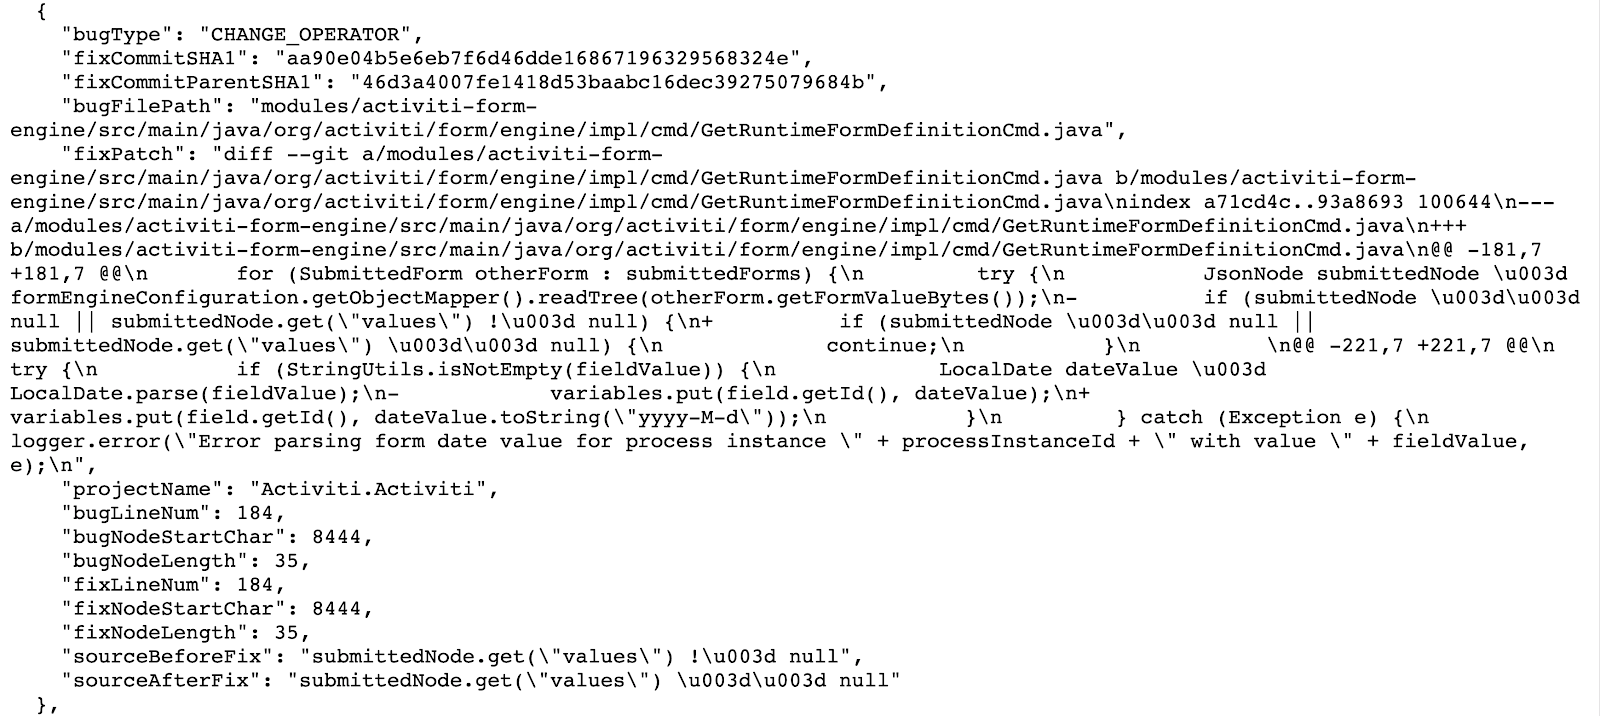
\includegraphics[width=\linewidth]{img/dataset_snap.png}
	\begingroup
	\fontsize{7pt}{10pt}\selectfont
	\begin{verbatim}
{
"bugType": "CHANGE_OPERATOR",
"fixCommitSHA1": "aa90e04b5e6eb7f6d46dde16867196329568324e",
"fixCommitParentSHA1": "46d3a4007fe1418d53baabc16dec39275079684b",
"bugFilePath": "/java/org/../GetRuntimeFormDefinitionCmd.java",
"fixPatch": "...",
"projectName": "Activiti.Activiti",
"bugLineNum": 184,
"bugNodeStartChar": 8444,
"bugNodeLength": 35,
"fixLineNum": 184,
"fixNodeStartChar": 8444,
"fixNodeLength": 35,
"sourceBeforeFix": "submittedNode.get(\"values\") != null",
"sourceAfterFix": "submittedNode.get(\"values\") == null"
}
	\end{verbatim}
	\endgroup
	\caption{Dataset item Snap}
	\Description{A snap of a single databest item.}
	\label{fig:database_snap}
\end{figure}

Table \ref{tab:stat}, shows the dataset statistics. This dataset contains 100 Java Maven and 100 other Java projects. We have used the maven projects for our experiments.
\begin{table}[h]
	\begin{tabular}{|c|c|c|c|c|}
		\hline
		\textbf{Projects}&\textbf{Bug}&\textbf{Buggy}&\textbf{Bugs}&\textbf{SStuBs}\\
		& \textbf{Commits}&  \textbf{stmts} & \textbf{per}&\\
		& & & \textbf{Commit}&\\
		\hline
		100 Java Maven&12598		   & 25539	&	          2.03    &  		7824\\
		100 Java&86771   	   & 153652	&	          1.77     &  		51537\\
		\hline
	\end{tabular}
	\caption{Statistics of Dataset}
	\label{tab:stat}
\end{table}

Besides automated scripts, we have worked on manual projects to generate the test coverage reports for the projects. Figure \ref{fig:method_snap} shows our overall methodology.

\begin{figure}[h]
	\centering
	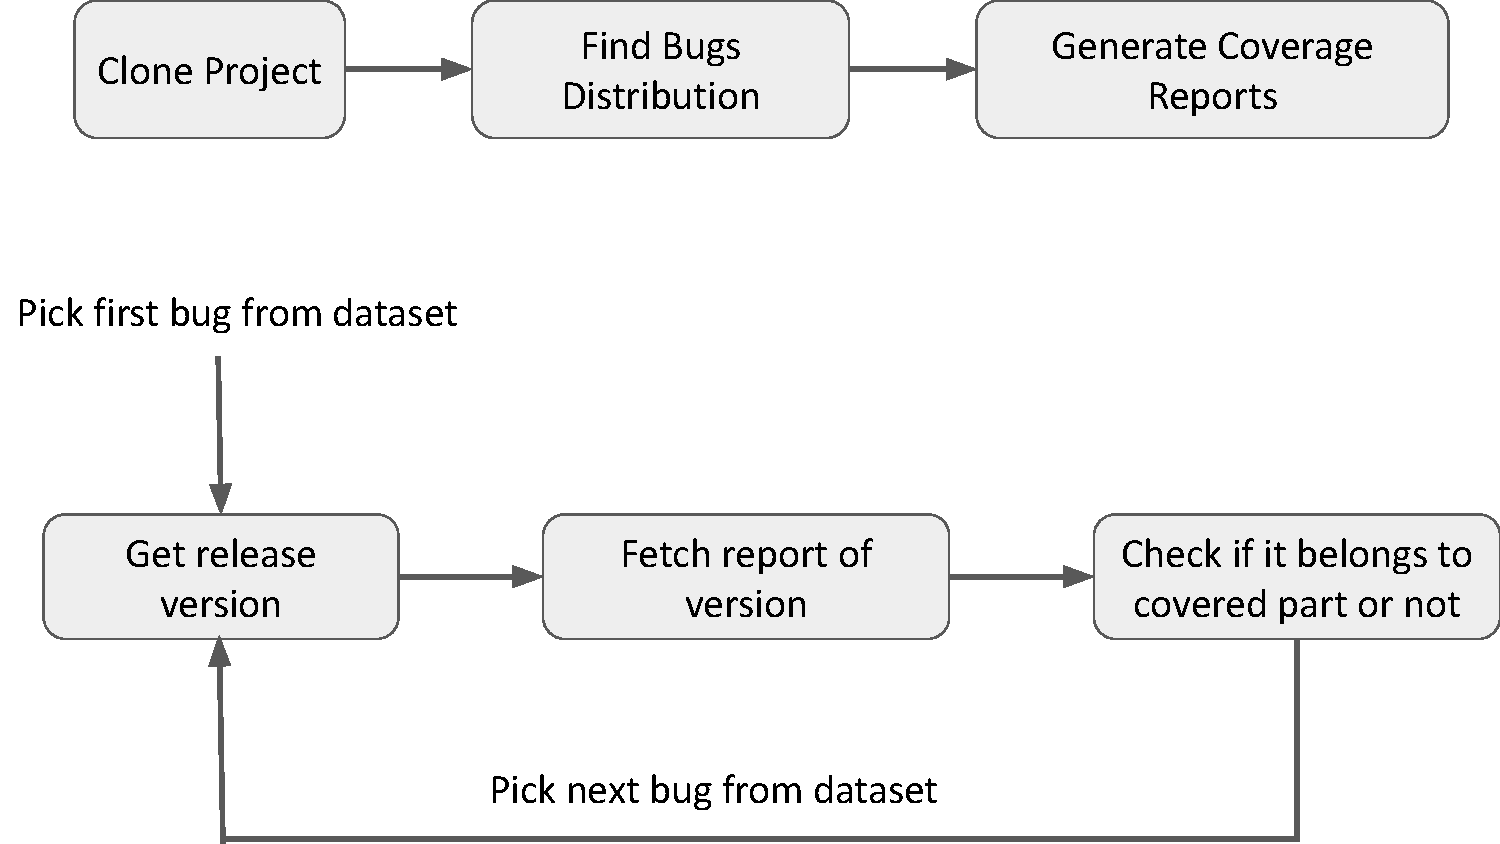
\includegraphics[width=1.0\linewidth]{img/method.pdf}
	\caption{Overall Methodology}
	\Description{A snap of overall methodology.}
	\label{fig:method_snap}
\end{figure}

\subsection{Split ProjectWise Dataset}
We have separated the dataset based on the project. Firstly, we have sorted the dataset based on the project name and then split the JSON array into separate JSON files. In each of the new datasets, they contain bugs from the same project.
\subsection{Clone Project}
We cloned the projects from Github depending on the project name. We used $SSH$ repository links. We have run $git\ clone\ repo\_link$ and save those repository in our local machine. In the dataset, the project name contains the username or the organization name appended by the repository name in Github.
\subsection{Find the Distribution of Bugs}
For each project, we then calculate the number of bugs per year to identify the period where maximum number of single statement bugs occur. Figures \ref{fig:distribution} show an example of bug frequency distribution.

\begin{figure}[h]
	\centering
	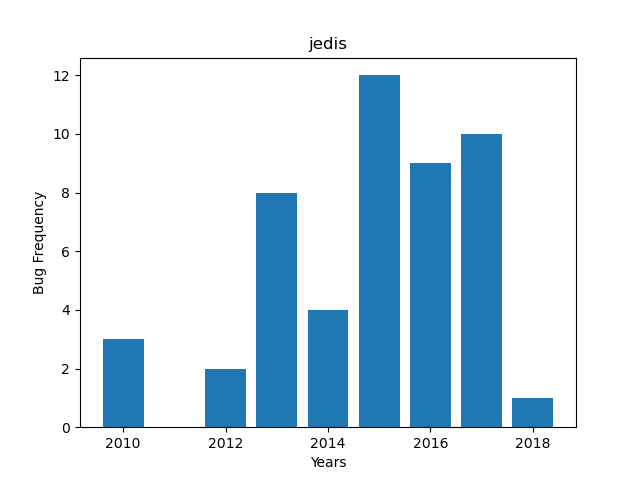
\includegraphics[width=0.6\linewidth]{img/freq.png}
	\caption{Frequency of SSBs in a project named "jedis"}% on GitHub using Maven build system}
	\Description{A graph of frequency of SSBs over the years}
	\label{fig:distribution}
\end{figure}

\subsection{Generate Coverage Report}
Each of the projects are depended on various of software tools and packages. Some of the packages are already depreciated. So, we had manually check each of the project version to fix the dependencies and run the test on specific version for every project. Later, with the updated $pom.xml$ file, we run $"mvn\ clean\ test"$ to generate the coverage report. From the generated coverage report artifacts, we used the $jacoco.xml, index.html$ files under the report directory.

\subsection{Get Release Versions} To fetch the project version with high frequency of SSB, we analyzed all release version. We had considered a project version with it's release tag. We checkout each version of the project based on the tags. We used the common $git\ checkout\ version\_name$ command for this task.
\subsection{Fetch Report for Project Version}
In previous "Generate Coverage Report" stage, we generated code coverage reports manually. In this stage, we fetch those reports automatically based on the project version. In our report directory, we had stored the report with version name under the parent project name. Later on this stage, we loaded the $XML$ and $HTML$ reports in our system to count the bugs in covered part, not covered part, and average of percentage coverage.
\subsection{Count SSBs in Covered, Not Covered Part, and Average Percentage Coverage}
In this step, we count the number of bugs in covered and not covered part from the $jacoco.xml$ report by parsing the $XML$. In addition to that, we count the average percentage of coverage from the $index.html$ report from JACOCO. %Figure () shows the XML report snap where it indicates the bug line number and the coverage state.
\subsection{Calculate the Correlation Coefficient}
In this final step of methodology, we calculated the correlation coefficient between the percentage of bugs that are not covered part and the average percentage coverage. We used the Equation \ref{eq:1} for the calculation. Based on this correlation coefficient, we verified out hypothesis.
\subsection{Experimental Setup} Our experiments were run on a Linux machine with Ubuntu 20.04 LTS OS version. For cloning Github projects, we have used bash and python3. To generate coverage reports, we had used the project depended package version of Java and other software packages.

To parse XML and HTML report, we had used several packages like $xml.dom.minidom, bs4$. We had used $matplotlib.pyplot$ to plot necessary graphs for our experiments.

\section{Results}
Previous section explains how we used the SStuBs to collect the data from GitHub, used Jacoco to generate the coverage reports, and processed them to get the desired data. In this section, using that data, we try to answer our research question.

\subsection{How is testing related to SSBs?}

In our research question, we asked if there a correlation between test coverage and SSBs. The purpose of this question is to find out if increasing the coverage can be “actually” helpful in reducing the SSBs.

\begin{table}[H]
	\begin{tabular}{|c|c|c|}
		\hline
		\textbf{Project Name} & \textbf{Percentage} & \textbf{Bugs in Not} \\
		&\textbf{Coverage}& \textbf{Covered (\%)}\\
		\hline
		alibaba.druid &41.67&58.33\\
		alibaba.fastjson & 50&	50\\
		AsyncHttpClient.async-http-client &40&60\\
		brettwooldridge.HikariCP &5.88&	94.12\\
		Bukkit.Bukkit &68&32\\
		cucumber.cucumber-jvm &50&50\\
		google.auto &19.23&80.769\\
		google.closure-compiler &52.38&	47.62\\
		google.guice&35&65\\
		jhy.jsoup&45.45&54.55\\
		junit-team.junit &18.75&81.25\\
		mybatis.mybatis-3 &16.67&83.33\\
		\hline
	\end{tabular}
	\caption{Data collected about projects on percentage coverage and percentage of SSBs in not covered part}
	\label{tab:ppc}
\end{table}

Table \ref{tab:ppc}  shows the data collected to answer this question. The first column shows the project name, and the second column shows the average percentage test coverage, while the third column shows the percentage of SSBs in the not covered part. We are considering the bugs in the non-covered part as they provide an easy way to understand the effectiveness of coverage. A higher percentage of them indicates that coverage is effective and vice versa. In our data, we have a mixed percentage. We used this data to find the correlation coefficient (\emph{r}) between the percentage of coverage and the percentage of SSBs. The \emph{r}-value turned out to be 0.40, which translates into a weak to moderate positive correlation between them. It shows that high coverage helps mitigate the SSBs. This correlation is shown in \ref{fig:corr}. We can see that increased covered is related to greater percentage of bugs in the not covered part and testing is useful here.\\


\begin{figure}[h]
	\centering
	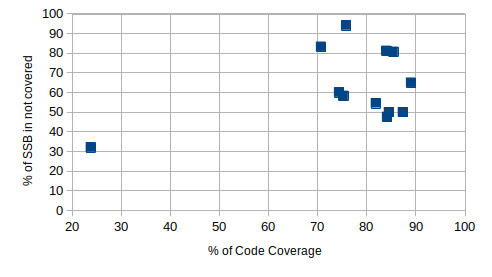
\includegraphics[width=\linewidth]{img/correlation.png}
	\caption{Correlation of the percentage of bugs in not covered part and the average of percentage test coverage}
	\label{fig:corr}
\end{figure}



\fbox{\begin{minipage}{25em}
		\textbf{RQ 1 Answer.} \emph{Our results suggest that there is a positive weak to moderate correlation between the unit test coverage and the number of SSBs found in the not covered parts. The coverage seems to be effective for SSBs, to some degree.}
	\end{minipage}}\\\\



Our study has a few important implications. Firstly, it is one of its kind to explore the effectiveness of coverage on the SSBs and the results indicate that it’s a promising research area to further investigate. Further studies will help better understand the nature of this relationship under different settings and we might be able to reach a consensus about the unit test effectiveness. Secondly, knowing that testing is helpful, will help the practitioners allocate resources and prioritize testing more effectively. Which in turn, can help improve the software quality.


\section{Threats to the validity}
In this section, we discuss some of the possible threats to the validity of our study. As described in section 4, we considered multiple versions of each project and wrote our scripts for processing and some tasks automation. This involvement of the human factor equates to the possibility of human error in the process. There could be a mismatch in the versions, and we could have made some unintentional mistakes in the code, however, throughout the process we also did manual verification to reduce this risk. The results of our study are also limited by the SStuBs(sstubs) dataset we used. While it includes a good number and range of projects from different domains, it is limited by the language type and build system. All the projects use the Maven build system and are developed in Java. The results obtained from the study might not apply to the other type system, languages, or even other build systems.

Another important aspect to consider is that all the reports are generated manually by checking out each version one by one, resolving dependencies, and configuring Jacoco. It is not only a tedious manual process but also makes it highly susceptible to error. However, throughout the process, we did manual verification to mitigate this threat as much as possible. Another threat is that the projects included in the dataset are the top open-source Java projects. They are maintained for more than a decade by the open-source community and used by tons of organizations and developers. Through their feedback and community involvement, they have matured over the years. Since we only consider the high-density bugs areas where we have tests written and we can generate reports, they might not reflect their whole project life cycle. Lastly, since we only considered open source projects, our results might not apply to the close source projects.

\section{Conclusion and Future Work}

%\section{Typefaces}
%
%The ``\verb|acmart|'' document class requires the use of the
%``Libertine'' typeface family. Your \TeX\ installation should include
%this set of packages. Please do not substitute other typefaces. The
%``\verb|lmodern|'' and ``\verb|ltimes|'' packages should not be used,
%as they will override the built-in typeface families.
%
%\section{Title Information}
%
%The title of your work should use capital letters appropriately -
%\url{https://capitalizemytitle.com/} has useful rules for
%capitalization. Use the {\verb|title|} command to define the title of
%your work. If your work has a subtitle, define it with the
%{\verb|subtitle|} command.  Do not insert line breaks in your title.
%
%If your title is lengthy, you must define a short version to be used
%in the page headers, to prevent overlapping text. The \verb|title|
%command has a ``short title'' parameter:
%\begin{verbatim}
%  \title[short title]{full title}
%\end{verbatim}
%
%\section{Authors and Affiliations}
%
%Each author must be defined separately for accurate metadata
%identification. Multiple authors may share one affiliation. Authors'
%names should not be abbreviated; use full first names wherever
%possible. Include authors' e-mail addresses whenever possible.
%
%Grouping authors' names or e-mail addresses, or providing an ``e-mail
%alias,'' as shown below, is not acceptable:
%\begin{verbatim}
%  \author{Brooke Aster, David Mehldau}
%  \email{dave,judy,steve@university.edu}
%  \email{firstname.lastname@phillips.org}
%\end{verbatim}
%
%The \verb|authornote| and \verb|authornotemark| commands allow a note
%to apply to multiple authors --- for example, if the first two authors
%of an article contributed equally to the work.
%
%If your author list is lengthy, you must define a shortened version of
%the list of authors to be used in the page headers, to prevent
%overlapping text. The following command should be placed just after
%the last \verb|\author{}| definition:
%\begin{verbatim}
%  \renewcommand{\shortauthors}{McCartney, et al.}
%\end{verbatim}
%Omitting this command will force the use of a concatenated list of all
%of the authors' names, which may result in overlapping text in the
%page headers.
%
%The article template's documentation, available at
%\url{https://www.acm.org/publications/proceedings-template}, has a
%complete explanation of these commands and tips for their effective
%use.
%
%Note that authors' addresses are mandatory for journal articles.
%
%\section{Rights Information}
%
%Authors of any work published by ACM will need to complete a rights
%form. Depending on the kind of work, and the rights management choice
%made by the author, this may be copyright transfer, permission,
%license, or an OA (open access) agreement.
%
%Regardless of the rights management choice, the author will receive a
%copy of the completed rights form once it has been submitted. This
%form contains \LaTeX\ commands that must be copied into the source
%document. When the document source is compiled, these commands and
%their parameters add formatted text to several areas of the final
%document:
%\begin{itemize}
%\item the ``ACM Reference Format'' text on the first page.
%\item the ``rights management'' text on the first page.
%\item the conference information in the page header(s).
%\end{itemize}
%
%Rights information is unique to the work; if you are preparing several
%works for an event, make sure to use the correct set of commands with
%each of the works.
%
%The ACM Reference Format text is required for all articles over one
%page in length, and is optional for one-page articles (abstracts).
%
%\section{CCS Concepts and User-Defined Keywords}
%
%Two elements of the ``acmart'' document class provide powerful
%taxonomic tools for you to help readers find your work in an online
%search.
%
%The ACM Computing Classification System ---
%\url{https://www.acm.org/publications/class-2012} --- is a set of
%classifiers and concepts that describe the computing
%discipline. Authors can select entries from this classification
%system, via \url{https://dl.acm.org/ccs/ccs.cfm}, and generate the
%commands to be included in the \LaTeX\ source.
%
%User-defined keywords are a comma-separated list of words and phrases
%of the authors' choosing, providing a more flexible way of describing
%the research being presented.
%
%CCS concepts and user-defined keywords are required for for all
%articles over two pages in length, and are optional for one- and
%two-page articles (or abstracts).
%
%\section{Sectioning Commands}
%
%Your work should use standard \LaTeX\ sectioning commands:
%\verb|section|, \verb|subsection|, \verb|subsubsection|, and
%\verb|paragraph|. They should be numbered; do not remove the numbering
%from the commands.
%
%Simulating a sectioning command by setting the first word or words of
%a paragraph in boldface or italicized text is {\bfseries not allowed.}
%
%\section{Tables}
%
%The ``\verb|acmart|'' document class includes the ``\verb|booktabs|''
%package --- \url{https://ctan.org/pkg/booktabs} --- for preparing
%high-quality tables.
%
%Table captions are placed {\itshape above} the table.
%
%Because tables cannot be split across pages, the best placement for
%them is typically the top of the page nearest their initial cite.  To
%ensure this proper ``floating'' placement of tables, use the
%environment \textbf{table} to enclose the table's contents and the
%table caption.  The contents of the table itself must go in the
%\textbf{tabular} environment, to be aligned properly in rows and
%columns, with the desired horizontal and vertical rules.  Again,
%detailed instructions on \textbf{tabular} material are found in the
%\textit{\LaTeX\ User's Guide}.
%
%Immediately following this sentence is the point at which
%Table~\ref{tab:freq} is included in the input file; compare the
%placement of the table here with the table in the printed output of
%this document.
%
%\begin{table}
%  \caption{Frequency of Special Characters}
%  \label{tab:freq}
%  \begin{tabular}{ccl}
%    \toprule
%    Non-English or Math&Frequency&Comments\\
%    \midrule
%    \O & 1 in 1,000& For Swedish names\\
%    $\pi$ & 1 in 5& Common in math\\
%    \$ & 4 in 5 & Used in business\\
%    $\Psi^2_1$ & 1 in 40,000& Unexplained usage\\
%  \bottomrule
%\end{tabular}
%\end{table}
%
%To set a wider table, which takes up the whole width of the page's
%live area, use the environment \textbf{table*} to enclose the table's
%contents and the table caption.  As with a single-column table, this
%wide table will ``float'' to a location deemed more
%desirable. Immediately following this sentence is the point at which
%Table~\ref{tab:commands} is included in the input file; again, it is
%instructive to compare the placement of the table here with the table
%in the printed output of this document.
%
%\begin{table*}
%  \caption{Some Typical Commands}
%  \label{tab:commands}
%  \begin{tabular}{ccl}
%    \toprule
%    Command &A Number & Comments\\
%    \midrule
%    \texttt{{\char'134}author} & 100& Author \\
%    \texttt{{\char'134}table}& 300 & For tables\\
%    \texttt{{\char'134}table*}& 400& For wider tables\\
%    \bottomrule
%  \end{tabular}
%\end{table*}
%
%Always use midrule to separate table header rows from data rows, and
%use it only for this purpose. This enables assistive technologies to
%recognise table headers and support their users in navigating tables
%more easily.
%
%\section{Math Equations}
%You may want to display math equations in three distinct styles:
%inline, numbered or non-numbered display.  Each of the three are
%discussed in the next sections.
%
%\subsection{Inline (In-text) Equations}
%A formula that appears in the running text is called an inline or
%in-text formula.  It is produced by the \textbf{math} environment,
%which can be invoked with the usual
%\texttt{{\char'134}begin\,\ldots{\char'134}end} construction or with
%the short form \texttt{\$\,\ldots\$}. You can use any of the symbols
%and structures, from $\alpha$ to $\omega$, available in
%\LaTeX~\cite{Lamport:LaTeX}; this section will simply show a few
%examples of in-text equations in context. Notice how this equation:
%\begin{math}
%  \lim_{n\rightarrow \infty}x=0
%\end{math},
%set here in in-line math style, looks slightly different when
%set in display style.  (See next section).
%
%\subsection{Display Equations}
%A numbered display equation---one set off by vertical space from the
%text and centered horizontally---is produced by the \textbf{equation}
%environment. An unnumbered display equation is produced by the
%\textbf{displaymath} environment.
%
%Again, in either environment, you can use any of the symbols and
%structures available in \LaTeX\@; this section will just give a couple
%of examples of display equations in context.  First, consider the
%equation, shown as an inline equation above:
%\begin{equation}
%  \lim_{n\rightarrow \infty}x=0
%\end{equation}
%Notice how it is formatted somewhat differently in
%the \textbf{displaymath}
%environment.  Now, we'll enter an unnumbered equation:
%\begin{displaymath}
%  \sum_{i=0}^{\infty} x + 1
%\end{displaymath}
%and follow it with another numbered equation:
%\begin{equation}
%  \sum_{i=0}^{\infty}x_i=\int_{0}^{\pi+2} f
%\end{equation}
%just to demonstrate \LaTeX's able handling of numbering.
%
%\section{Figures}
%
%The ``\verb|figure|'' environment should be used for figures. One or
%more images can be placed within a figure. If your figure contains
%third-party material, you must clearly identify it as such, as shown
%in the example below.
%\begin{figure}[h]
%  \centering
%  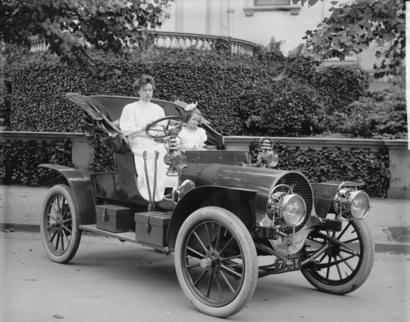
\includegraphics[width=\linewidth]{sample-franklin}
%  \caption{1907 Franklin Model D roadster. Photograph by Harris \&
%    Ewing, Inc. [Public domain], via Wikimedia
%    Commons. (\url{https://goo.gl/VLCRBB}).}
%  \Description{A woman and a girl in white dresses sit in an open car.}
%\end{figure}
%
%Your figures should contain a caption which describes the figure to
%the reader.
%
%Figure captions are placed {\itshape below} the figure.
%
%Every figure should also have a figure description unless it is purely
%decorative. These descriptions convey what’s in the image to someone
%who cannot see it. They are also used by search engine crawlers for
%indexing images, and when images cannot be loaded.
%
%A figure description must be unformatted plain text less than 2000
%characters long (including spaces).  {\bfseries Figure descriptions
%  should not repeat the figure caption – their purpose is to capture
%  important information that is not already provided in the caption or
%  the main text of the paper.} For figures that convey important and
%complex new information, a short text description may not be
%adequate. More complex alternative descriptions can be placed in an
%appendix and referenced in a short figure description. For example,
%provide a data table capturing the information in a bar chart, or a
%structured list representing a graph.  For additional information
%regarding how best to write figure descriptions and why doing this is
%so important, please see
%\url{https://www.acm.org/publications/taps/describing-figures/}.
%
%\subsection{The ``Teaser Figure''}
%
%A ``teaser figure'' is an image, or set of images in one figure, that
%are placed after all author and affiliation information, and before
%the body of the article, spanning the page. If you wish to have such a
%figure in your article, place the command immediately before the
%\verb|\maketitle| command:
%\begin{verbatim}
%  \begin{teaserfigure}
%    \includegraphics[width=\textwidth]{sampleteaser}
%    \caption{figure caption}
%    \Description{figure description}
%  \end{teaserfigure}
%\end{verbatim}
%
%\section{Citations and Bibliographies}
%
%The use of \BibTeX\ for the preparation and formatting of one's
%references is strongly recommended. Authors' names should be complete
%--- use full first names (``Donald E. Knuth'') not initials
%(``D. E. Knuth'') --- and the salient identifying features of a
%reference should be included: title, year, volume, number, pages,
%article DOI, etc.
%
%The bibliography is included in your source document with these two
%commands, placed just before the \verb|\end{document}| command:
%\begin{verbatim}
%  \bibliographystyle{ACM-Reference-Format}
%  \bibliography{bibfile}
%\end{verbatim}
%where ``\verb|bibfile|'' is the name, without the ``\verb|.bib|''
%suffix, of the \BibTeX\ file.
%
%Citations and references are numbered by default. A small number of
%ACM publications have citations and references formatted in the
%``author year'' style; for these exceptions, please include this
%command in the {\bfseries preamble} (before the command
%``\verb|\begin{document}|'') of your \LaTeX\ source:
%\begin{verbatim}
%  \citestyle{acmauthoryear}
%\end{verbatim}
%
%  Some examples.  A paginated journal article \cite{Abril07}, an
%  enumerated journal article \cite{Cohen07}, a reference to an entire
%  issue \cite{JCohen96}, a monograph (whole book) \cite{Kosiur01}, a
%  monograph/whole book in a series (see 2a in spec. document)
%  \cite{Harel79}, a divisible-book such as an anthology or compilation
%  \cite{Editor00} followed by the same example, however we only output
%  the series if the volume number is given \cite{Editor00a} (so
%  Editor00a's series should NOT be present since it has no vol. no.),
%  a chapter in a divisible book \cite{Spector90}, a chapter in a
%  divisible book in a series \cite{Douglass98}, a multi-volume work as
%  book \cite{Knuth97}, a couple of articles in a proceedings (of a
%  conference, symposium, workshop for example) (paginated proceedings
%  article) \cite{Andler79, Hagerup1993}, a proceedings article with
%  all possible elements \cite{Smith10}, an example of an enumerated
%  proceedings article \cite{VanGundy07}, an informally published work
%  \cite{Harel78}, a couple of preprints \cite{Bornmann2019,
%    AnzarootPBM14}, a doctoral dissertation \cite{Clarkson85}, a
%  master's thesis: \cite{anisi03}, an online document / world wide web
%  resource \cite{Thornburg01, Ablamowicz07, Poker06}, a video game
%  (Case 1) \cite{Obama08} and (Case 2) \cite{Novak03} and \cite{Lee05}
%  and (Case 3) a patent \cite{JoeScientist001}, work accepted for
%  publication \cite{rous08}, 'YYYYb'-test for prolific author
%  \cite{SaeediMEJ10} and \cite{SaeediJETC10}. Other cites might
%  contain 'duplicate' DOI and URLs (some SIAM articles)
%  \cite{Kirschmer:2010:AEI:1958016.1958018}. Boris / Barbara Beeton:
%  multi-volume works as books \cite{MR781536} and \cite{MR781537}. A
%  couple of citations with DOIs:
%  \cite{2004:ITE:1009386.1010128,Kirschmer:2010:AEI:1958016.1958018}. Online
%  citations: \cite{TUGInstmem, Thornburg01, CTANacmart}. Artifacts:
%  \cite{R} and \cite{UMassCitations}.

%\section{Acknowledgments}
%
%Identification of funding sources and other support, and thanks to
%individuals and groups that assisted in the research and the
%preparation of the work should be included in an acknowledgment
%section, which is placed just before the reference section in your
%document.
%
%This section has a special environment:
%\begin{verbatim}
%  \begin{acks}
%  ...
%  \end{acks}
%\end{verbatim}
%so that the information contained therein can be more easily collected
%during the article metadata extraction phase, and to ensure
%consistency in the spelling of the section heading.
%
%Authors should not prepare this section as a numbered or unnumbered {\verb|\section|}; please use the ``{\verb|acks|}'' environment.

%\section{Appendices}
%
%If your work needs an appendix, add it before the
%``\verb|\end{document}|'' command at the conclusion of your source
%document.
%
%Start the appendix with the ``\verb|appendix|'' command:
%\begin{verbatim}
%  \appendix
%\end{verbatim}
%and note that in the appendix, sections are lettered, not
%numbered. This document has two appendices, demonstrating the section
%and subsection identification method.
%
%\section{SIGCHI Extended Abstracts}
%
%The ``\verb|sigchi-a|'' template style (available only in \LaTeX\ and
%not in Word) produces a landscape-orientation formatted article, with
%a wide left margin. Three environments are available for use with the
%``\verb|sigchi-a|'' template style, and produce formatted output in
%the margin:
%\begin{itemize}
%\item {\verb|sidebar|}:  Place formatted text in the margin.
%\item {\verb|marginfigure|}: Place a figure in the margin.
%\item {\verb|margintable|}: Place a table in the margin.
%\end{itemize}

%%
%% The acknowledgments section is defined using the "acks" environment
%% (and NOT an unnumbered section). This ensures the proper
%% identification of the section in the article metadata, and the
%% consistent spelling of the heading.
% \begin{acks}
% To Robert, for the bagels and explaining CMYK and color spaces.
% \end{acks}

%%
%% The next two lines define the bibliography style to be used, and
%% the bibliography file.
\bibliographystyle{ACM-Reference-Format}
\bibliography{sample-base}

%%
%% If your work has an appendix, this is the place to put it.
\appendix

%\section{Research Methods}
%
%\subsection{Part One}
%
%Lorem ipsum dolor sit amet, consectetur adipiscing elit. Morbi
%malesuada, quam in pulvinar varius, metus nunc fermentum urna, id
%sollicitudin purus odio sit amet enim. Aliquam ullamcorper eu ipsum
%vel mollis. Curabitur quis dictum nisl. Phasellus vel semper risus, et
%lacinia dolor. Integer ultricies commodo sem nec semper.
%
%\subsection{Part Two}
%
%Etiam commodo feugiat nisl pulvinar pellentesque. Etiam auctor sodales
%ligula, non varius nibh pulvinar semper. Suspendisse nec lectus non
%ipsum convallis congue hendrerit vitae sapien. Donec at laoreet
%eros. Vivamus non purus placerat, scelerisque diam eu, cursus
%ante. Etiam aliquam tortor auctor efficitur mattis.
%
%\section{Online Resources}
%
%Nam id fermentum dui. Suspendisse sagittis tortor a nulla mollis, in
%pulvinar ex pretium. Sed interdum orci quis metus euismod, et sagittis
%enim maximus. Vestibulum gravida massa ut felis suscipit
%congue. Quisque mattis elit a risus ultrices commodo venenatis eget
%dui. Etiam sagittis eleifend elementum.
%
%Nam interdum magna at lectus dignissim, ac dignissim lorem
%rhoncus. Maecenas eu arcu ac neque placerat aliquam. Nunc pulvinar
%massa et mattis lacinia.

\end{document}
\endinput
%%
%% End of file `sample-manuscript.tex'.
